\chapter{Easy Hyperparameter Search Using Optunity}\label{ch:optunity}

\hyphenation{Optunity}
\newcommand{\optunity}{{\sc Optunity}\xspace}

\chapterfrontpagesubmitted{
Claesen, M., Simm, J., Popovic, D., Moreau, Y., \& De Moor, B. (2015). 
\textbf{Easy hyperparameter search using Optunity},
\emph{Journal of Machine Learning Research}.
}{
Marc Claesen has developed, maintained, tested and documented the software in Python, MATLAB and Octave and took the lead in writing the initial draft, the revision and rebuttal of the paper.
}{
    \optunity is a free software package dedicated to hyperparameter optimization. It contains various types of solvers, ranging from undirected methods to direct search, particle swarm and evolutionary optimization. The design focuses on ease of use, flexibility, code clarity and interoperability with existing software in popular machine learning environments. \optunity is written in Python and contains interfaces to R, Octave and MATLAB.  \optunity uses a BSD license and is available at \texttt{\url{http://www.optunity.net}}.
}

\section{Introduction}
Many machine learning tasks involve training a model $\mathcal{M}$ which minimizes some loss function $\mathcal{L}(\mathcal{M}\ |\ \test)$ on given test data $\test$. A model is obtained via a learning algorithm $\mathcal{A}$ which uses a training set $\train$ and solves some optimization problem. The learning algorithm $\mathcal{A}$ may itself be parameterized by a set of hyperparameters $\lambda$, e.g. $\mathcal{M} = \mathcal{A}(\train\ |\ \lambda)$.  Hyperparameter search -- also known as tuning -- aims to find a set of hyperparameters $\lambda^*$, such that the learning algorithm yields an optimal model $\mathcal{M}^*$ that minimizes $\mathcal{L}(\mathcal{M}\ |\ \test)$:
\begin{equation}
\lambda^* = \argmin_{\lambda} \mathcal{L}\big(\mathcal{A}(\train\ |\ \lambda)\ |\ \test\big) = \argmin_{\lambda} \obj(\lambda\ |\ \mathcal{A},\ \train, \test,\ \mathcal{L}). \label{equation}
\end{equation}
In tuning, $\obj$ is the objective function and the hyperparameters $\lambda$ are optimization variables. The learning algorithm $\mathcal{A}$, loss function $\mathcal{L}$ and data sets $\train$ and $\test$ are known. %Depending on the learning task, $\train$ and $\test$ may be labeled and/or equal to each other. The objective function often has a constrained domain (for example regularization terms must be positive) and is assumed to be expensive to evaluate, black-box and non-smooth.

Tuning hyperparameters is a recurrent task in machine learning which may significantly affect overall performance. Commonly tuned hyperparameters are related to kernels, regularization, learning rates and network architecture. Some specific challenges associated to hyperparameter optimization are discussed by Claesen and De Moor \citep{claesen2015hyperparameter}. General machine learning packages provide only basic tuning methods like grid search \citep{pedregosa2011scikit}. In practice, the most common tuning approaches are grid search and manual tuning, though both are known to fail when the number of hyperparameters grows and manual search is additionally hard to reproduce \citep{bergstra2012random}.

\section{Optunity}
\optunity offers various optimizers and utility functions to enable efficient hyperparameter optimization using only a few of lines of code and minimal expertise. Our software is complementary to libraries that provide learning algorithms, such as \textsc{scikit-learn} \citep{pedregosa2011scikit}. The package uses a BSD license and is simple to deploy in any environment. \optunity supports Python, R, Octave and MATLAB on Linux, OSX and Windows.

\subsection{Functional Overview}
\optunity provides both simple routines for lay users and expert routines that enable fine-grained control of various aspects of the solving process. Basic tuning requires only an objective function, a maximum number of evaluations and box constraints on the hyperparameters to be optimized. Conditional search spaces in which the existence of some hyperparameters is contingent upon some discrete choice are also supported.

The objective function must be defined by the user. It takes a hyperparameter tuple $\lambda$ and typically involves three steps: (i) training a model $\mathcal{M}$ with $\lambda$, (ii) use $\mathcal{M}$ to predict a test set and (iii) compute some score or loss based on the predictions. %In unsupervised tasks, the separation between (i) and (ii) need not exist, for example in clustering a data set.

Tuning involves a series of function evaluations until convergence or until a predefined maximum number of evaluations is reached. \optunity is capable of vectorizing evaluations in the working environment to speed up the process at the end user's volition.

\optunity also provides $k$-fold cross-validation to estimate the generalization performance of supervised modeling approaches. The implementation can account for strata and clusters.\footnote{Instances in a stratum should be spread across folds. Clustered instances must remain in a single fold.} Finally, a variety of common quality metrics is available. 
The snippet below shows how to tune an SVM classifier with RBF kernel using {\sc scikit-learn} and \optunity:\footnote{We assume the correct imports are made and \texttt{data} and \texttt{labels} contain appropriate content.}


\begin{lstlisting}[style=Py, frame=none, xleftmargin=1.5ex, escapeinside={(*@}{@*)}]
!@optunity.cross_validated!(x=(*@\textcolor{red}{data}@*), y=(*@\textcolor{red}{labels}@*), num_folds=10, num_iter=2)
def (*@\textcolor{blue}{score}@*)(x_train, y_train, x_test, y_test, (*@\textcolor{blue}{C}@*), (*@\textcolor{blue}{gamma}@*)):
    model = sklearn.svm.SVC(C=10**(*@\textcolor{blue}{C}@*), gamma=10**(*@\textcolor{blue}{gamma}@*)).fit(x_train, y_train)
    decision_values = model.decision_function(x_test)
    return !optunity.metrics.roc_auc!(y_test, decision_values)

!hps!, _, _ = !optunity.maximize!((*@\textcolor{blue}{score}@*), num_evals=100, (*@\textcolor{blue}{C=[-5, 2]}@*), (*@\textcolor{blue}{gamma=[-5, 0]}@*)) (*@\label{optunity-maximize}@*)
svm = sklearn.svm.SVC(C=10**!hps['C']!, gamma=10**!hps['gamma']!) (*@\label{train-tuned-svm1}@*)
svm.fit((*@\textcolor{red}{data}@*), (*@\textcolor{red}{labels}@*)) (*@\label{train-tuned-svm2}@*)
\end{lstlisting}

The objective function as per Equation~\eqref{equation} is defined on lines 1 to 5, where $\lambda = (C, \gamma)$, $\mathcal{A}$ is the SVM training algorithm and $\mathcal{L}$ is area under the ROC curve. We use $2\times$ iterated 10-fold cross-validation to estimate area under the ROC curve. Up to $100$ hyperparameter tuples are tested in an exponential search space, bounded by $10^{-5} < C < 10^2$ and $10^{-5} < \gamma < 10^0$ on line \ref{optunity-maximize}. Finally, an SVM with optimized hyperparameters is trained on lines \ref{train-tuned-svm1} and \ref{train-tuned-svm2}.


\subsection{Available Solvers}
\optunity provides a wide variety of solvers, ranging from basic, undirected methods like grid search, sobol sequences and random search \citep{bergstra2012random} to evolutionary methods such as particle swarm optimization \citep{kennedy2010particle}, the covariance matrix adaptation evolutionary strategy (CMA-ES) \citep{hansen2001completely}, tree-structured Parzen estimator \citep{bergstra2011algorithms} and the Nelder-Mead simplex. The default solver is particle swarm optimization, which performs well for a large variety of tuning tasks involving various learning algorithms. Additional solvers will be incorporated in the future.
 
\subsection{Software Design and Implementation}

The design philosophy of \optunity prioritizes code clarity over performance. This is justified by the fact that objective function evaluations constitute the performance bottleneck. 

In contrast to typical Python packages, we avoid dependencies to facilitate users working in non-Python environments (sometimes at the cost of performance). To prevent issues for users that are unfamiliar with Python, care is taken to ensure all code in \optunity works out of the box on any Python version above 2.7, without requiring tools like \texttt{2to3} to make explicit conversions. \optunity has optional dependencies on {\sc DEAP} \citep{fortin2012deap} and {\sc Hyperopt} \citep{bergstra2013hyperopt} for the CMA-ES and TPE solvers, respectively. 

A key aspect of \optunity's design is interoperability with external environments. This requires bidirectional communication between \optunity's Python back-end ($\mathcal{O}$) and the external environment ($\mathcal{E}$) and roughly involves three steps: (i) $\mathcal{E}\rightarrow\mathcal{O}$ solver configuration, (ii) $\mathcal{O}\leftrightarrow\mathcal{E}$ objective function evaluations and (iii) $\mathcal{O}\rightarrow\mathcal{E}$ solution and solver summary. To this end, \optunity can do straightforward communication with any environment via sockets using JSON messages as shown in Figure~\ref{fig:workflow}. Only some information must be communicated, big objects like data sets are never exchanged. To port \optunity to a new environment, a thin wrapper must be implemented to handle communication.

\begin{figure}[!h]
  \centering 
      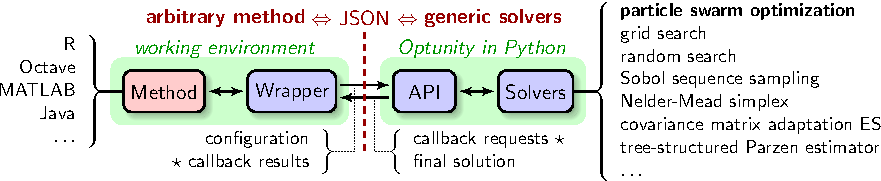
\includegraphics[width=\textwidth]{software.pdf} 
  \caption{Integrating \optunity in non-Python environments.}\label{fig:workflow}
\end{figure}

\subsection{Development and Documentation}
Collaborative development is organized via GitHub.\footnote{We maintain the following subdomains for convenience: \texttt{http://}$\{$\href{http://builds.optunity.net}{builds}, \href{http://docs.optunity.net}{docs}, \href{http://git.optunity.net}{git}, \href{http://issues.optunity.net}{issues}$\}$\texttt{.optunity.net}.} The project's master branch is kept stable and is subjected to continuous integration tests using Travis CI. 
We recommend prospective users to clone the master branch for the most up-to-date stable version of the software. Bug reports and feature requests can be filed via issues on GitHub. Future development efforts will focus on wrappers for Java and C/C++. We additionally plan to incorporate Bayesian optimizers which have no reference implementation in other packages. %Bayesian optimization strategies that are unavailable elsewhere \citep{jones1998efficient}. 

Code is documented using Sphinx and contains many doctests that can serve as both unit tests and examples of the associated functions. 
Our website contains developer and user documentation and a wide range of examples to illustrate all aspects of the software. 
The examples involve various packages and environments, including \textsc{scikit-learn} \citep{pedregosa2011scikit}, \textsc{OpenCV} \citep{opencv_library} and \textsc{Spark}'s \textsc{MLlib} \citep{zaharia2010spark}.
%Finally, some practical applications are available, including object recognition using OpenCV \citep{opencv_library} and deep learning with Theano \citep{bergstra2011theano}. % and semisupervised learning \citep{claesen2014robust}.

%\section{Conclusions}
%Optunity contains a variety of optimization methods that can be used for hyperparameter search. Using proper search methods becomes particularly important for machine learning methods with many hyperparameters, such as convolutional networks, deep belief networks and ensembles of SVM models.

\section{Related Work}

A number of software solutions exist for hyperparameter search. \textsc{Hyperopt} offers random search and sequential model-based optimization \citep{bergstra2013hyperopt}. Some packages dedicated to Bayesian approaches include \textsc{Spearmint} \citep{snoek2012practical}, \textsc{DiceKriging} \citep{roustant2012dicekriging}, \textsc{SMAC} \citep{hutter2011sequential} and \textsc{BayesOpt} \citep{martinez2014bayesopt}. Finally, \textsc{ParamILS} provides iterated local search \citep{hutter2009paramils}. 

%Existing packages tend to be one-trick ponies, providing a specific class of optimization methods and offering limited support to users in different machine learning environments. 
\optunity distinguishes itself from other packages by exposing a variety of fundamentally different solvers through a lightweight API. \optunity's client-server model facilitates integration in any language and environment and can even be used to run solvers remotely.

\section{Solver Benchmark}
We compared \textsc{Optunity} against \textsc{BayesOpt} \citep{martinez2014bayesopt}, \textsc{Hyperopt} \citep{bergstra2013hyperopt}, \textsc{SMAC} \citep{hutter2011sequential}, and random search \citep{bergstra2012random}. Implementations of the last three solvers were available in HPOlib \citep{eggensperger2013towards}. We optimized 5-fold cross-validated area under the ROC curve for an SVM classifier with an RBF kernel (with continuous hyperparameters $C$ and $\gamma$), given a fixed search space and a budget of 150 evaluations on 19 real-world problems. Each solver was given identical objective functions. Figures~\ref{fig:optunity-benchmark-75} and \ref{fig:optunity-benchmark-150} summarize the results using critical difference (CD) diagrams as introduced by Dem{\v{s}}ar \citep{demvsar2006statistical}. More detailed results are available in Appendix~\ref{optunity-appendix-benchmark}.\footnote{The benchmark implementation is available at \url{https://github.com/claesenm/optunity-benchmark}.}

\textsc{Optunity} and \textsc{BayesOpt} come out on top as they convincingly outperformed random search at 75 evaluations and took a notable lead over other solvers at 150 function evaluations, though the latter was not statistically significant. Overall, the results indicate that all directed optimizers are competitive and generally outperform random search.

%PSO has also been shown to be competitive to TPE in tuning RBMs by \citet{papa2015model}.

\begin{figure}[!h]
  \centering 
      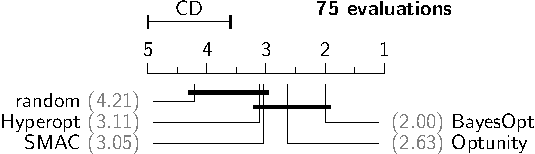
\includegraphics[width=0.8\textwidth]{cd_75.pdf}
\caption{Critical difference diagrams for 75 evaluations to tune an SVM with RBF kernel, depicting average rank per optimizer (lower is better). Optimizers with no statistically significant performance difference are linked with a horizontal bar.}\label{fig:optunity-benchmark-75}
\end{figure}

\begin{figure}[!h]
  \centering 
      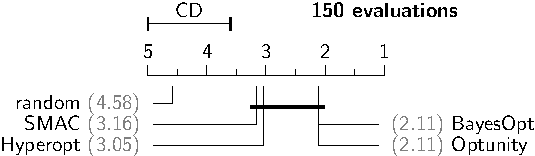
\includegraphics[width=0.8\textwidth]{cd_150.pdf}
\caption{Critical difference diagrams for 150 evaluations to tune an SVM with RBF kernel, depicting average rank per optimizer (lower is better). Optimizers with no statistically significant performance difference are linked with a horizontal bar.}\label{fig:optunity-benchmark-150}
\end{figure}


\begin{subappendices}

\section{Complete benchmark results} \label{optunity-appendix-benchmark}
In this benchmark we have optimized hyperparameters of an SVM classifier with RBF kernel on an exponential grid $10^{-8} < C < 10$ and $10^{-8} < \gamma < 10$. We used 5-fold cross-validation to estimate area under the ROC curve to build the objective function. All optimizers used the exact same objective function and a uniform prior to optimize $\log_{10}(C)$ and $\log_{10}(\gamma)$ within the specified bounds (the exponentiation was done within the objective function).

We simulated 19 real-world problems based on the \textsc{mnist}, \textsc{covtype}, \textsc{diabetes} and \textsc{ionosphere} data sets. Multiclass datasets were used several times in a one-vs-all setting, i.e., \textsc{mnist} and \textsc{covtype} were used to create 10 and 7 optimization problems, respectively. For some problems we added random noise on the data matrix to make the learning problems more challenging. 

Results of each optimization task at 75 and 150 evaluations are shown in Tables~\ref{table:benchmark-results-75} and \ref{table:benchmark-results-150}, respectively. Full code of all experiments is available at \url{https://github.com/claesenm/optunity-benchmark}.

\begin{table}[!h]
\centering
\begin{tabular}{lcccccc}
\toprule
dataset & Optunity & Hyperopt & SMAC & BayesOpt & random & $Q_3$ \\
\midrule
\texttt{digits-0} & \textbf{96.34} & 96.28 & 96.25 & 96.28 & 96.04 & 94.88 \\
\texttt{digits-1} & 92.40 & 92.36 & 91.92 & \textbf{92.60} & 91.78 & 87.28 \\
\texttt{digits-2} & 92.87 & 92.85 & \textbf{93.17} & 92.93 & 92.07 & 91.27 \\
\texttt{digits-3} & 90.51 & 90.12 & 90.21 & \textbf{90.87} & 90.44 & 89.06 \\
\texttt{digits-4} & 95.01 & 94.97 & 95.03 & \textbf{95.24} & 94.95 & 94.32 \\
\texttt{digits-5} & \textbf{94.90} & 94.50 & 94.52 & 94.65 & 94.33 & 93.13 \\
\texttt{digits-6} & 96.63 & \textbf{96.91} & 96.66 & 96.66 & 96.34 & 95.88 \\
\texttt{digits-7} & 95.03 & 94.81 & 95.22 & \textbf{95.35} & 94.31 & 93.32 \\
\texttt{digits-8} & 82.48 & \textbf{82.62} & 81.53 & 82.06 & 82.61 & 76.12 \\
\texttt{digits-9} & 86.77 & 86.89 & 87.09 & \textbf{87.32} & 86.26 & 84.05 \\
\texttt{covtype-1} & \textbf{81.62} & 81.07 & 80.74 & 80.74 & 80.80 & 77.02 \\
\texttt{covtype-2} & \textbf{80.41} & 79.41 & 79.37 & 79.37 & 78.10 & 74.24 \\
\texttt{covtype-3} & 97.01 & 97.47 & 97.37 & \textbf{97.73} & 97.35 & 94.01 \\
\texttt{covtype-4} & 99.93 & 99.80 & 99.92 & \textbf{99.94} & 99.91 & 98.54 \\
\texttt{covtype-5} & 95.99 & 95.50 & 95.74 & \textbf{96.12} & 95.66 & 89.02 \\
\texttt{covtype-6} & 96.73 & 97.14 & 97.12 & \textbf{97.53} & 97.30 & 92.59 \\
\texttt{covtype-7} & 98.06 & 97.77 & 97.48 & \textbf{98.28} & 97.90 & 94.03 \\
\texttt{diabetes} & 83.13 & 83.62 & \textbf{84.44} & 84.15 & 82.90 & 81.91 \\
\texttt{ionosphere} & 81.87 & \textbf{82.91} & 81.83 & 81.56 & 80.70 & 73.83 \\
\midrule
average rank & 2.632 & 3.105 & 3.053 & \textbf{2.000} & 4.211 & N/A \\
\bottomrule
\end{tabular}
\caption{Benchmark results for tuning an SVM classifier with RBF kernel, using 5-fold cross-validation and an optimization budget of 75 evaluations. Results depict each solver's optimum, which is cross-validated area under the ROC curve (in \%). Average rank indicates non-parametric global performance (lower is better). The last column shows the third quantile $Q_3$ of random search results, indicating the difficulty of the optimization problem: low $Q_3$ vis-\`a-vis the optimum indicates the region of strong performance is small within the overall search space.}
\label{table:benchmark-results-75}
\end{table}

\begin{table}[!h]
\centering
\begin{tabular}{lcccccc}
\toprule
dataset & Optunity & Hyperopt & SMAC & BayesOpt & random & $Q_3$ \\
\midrule
\texttt{digits-0} & 96.43 & 96.28 & 96.29 & \textbf{96.54} & 96.04 & 94.88 \\
\texttt{digits-1} & 92.40 & 92.69 & 92.19 & \textbf{93.21} & 92.21 & 87.28 \\
\texttt{digits-2} & \textbf{93.27} & 92.87 & 93.17 & 93.10 & 92.34 & 91.27 \\
\texttt{digits-3} & 90.69 & 90.54 & 90.59 & \textbf{90.87} & 90.44 & 89.06 \\
\texttt{digits-4} & \textbf{95.39} & 95.34 & 95.13 & 95.24 & 94.95 & 94.32 \\
\texttt{digits-5} & \textbf{94.90} & 94.50 & 94.67 & 94.65 & 94.33 & 93.13 \\
\texttt{digits-6} & 96.71 & \textbf{96.91} & 96.66 & 96.66 & 96.84 & 95.88 \\
\texttt{digits-7} & 95.11 & 95.10 & 95.22 & \textbf{95.36} & 94.54 & 93.32 \\
\texttt{digits-8} & \textbf{83.44} & 82.62 & 82.08 & 82.19 & 82.61 & 76.12 \\
\texttt{digits-9} & \textbf{87.49} & 87.22 & 87.09 & 87.32 & 86.50 & 84.05 \\
\texttt{covtype-1} & 82.24 & 81.89 & \textbf{82.43} & \textbf{82.43} & 80.80 & 77.02 \\
\texttt{covtype-2} & \textbf{81.18} & 80.41 & 80.33 & 80.33 & 78.52 & 74.24 \\
\texttt{covtype-3} & 97.55 & 97.51 & 97.37 & \textbf{97.76} & 97.35 & 94.01 \\
\texttt{covtype-4} & 99.93 & 99.91 & 99.92 & \textbf{99.94} & 99.91 & 98.54 \\
\texttt{covtype-5} & 95.99 & 95.67 & 95.74 & \textbf{96.38} & 95.66 & 89.02 \\
\texttt{covtype-6} & \textbf{97.59} & 97.52 & 97.39 & \textbf{97.59} & 97.30 & 92.59 \\
\texttt{covtype-7} & 98.23 & 98.00 & 97.88 & \textbf{98.36} & 97.90 & 94.03 \\
\texttt{diabetes} & 83.33 & 84.21 & \textbf{84.44} & 84.29 & 83.25 & 81.91 \\
\texttt{ionosphere} & 81.87 & \textbf{82.91} & 82.42 & 81.99 & 81.16 & 73.83 \\
\midrule
average rank & \textbf{2.105} & 3.053 & 3.158 & \textbf{2.105} & 4.579 & N/A \\
\bottomrule
\end{tabular}
\caption{Benchmark results for tuning an SVM classifier with RBF kernel, using 5-fold cross-validation and an optimization budget of 150 evaluations. Results depict each solver's optimum, which is cross-validated area under the ROC curve (in \%). Average rank indicates non-parametric global performance (lower is better). The last column shows the third quantile $Q_3$ of random search results, indicating the difficulty of the optimization problem: low $Q_3$ vis-\`a-vis the optimum indicates the region of strong performance is small within the overall search space.}
\label{table:benchmark-results-150}
\end{table}

\end{subappendices}

%%%%%%%%%%%%%%%%%%%%%%%%%%%%%%%%%%%%%%%%%%%%%%%%%%
% Keep the following \cleardoublepage at the end of this file, 
% otherwise \includeonly includes empty pages.
\cleardoublepage

% vim: tw=70 nocindent expandtab foldmethod=marker foldmarker={{{}{,}{}}}
